\chapter{System Overview and Data Flow}


[Intro Paragraph here.]


\section{Prototype System Overview}
The end to end camera system, as shown in figure 3.1 can be divided into 4 major stages by energy consumption, viz., image sensor, image signal processor(ISP), processor, and Off-chip memory. For our prototype camera design we use six IMX-274 cameras for capture and Nvidia Jetson TX2 for supporting camera capture and processing. The Camera and Jetson specs are shown in figure 3.2. 

Prototype System Overview\newline
Hardware:
System 1) Six Camera Rig for OmniDrirectional Stereo\newline
System 2) Dual Fisheye Camera for monoscopic 360 \newline
Software:
Nvidia libargus Camera API,
openCV, C++ \newline
Data Flow \newline

\section{Data Flow}
Block Diagram
- With different stages.
- With Data Inputs and Data Outputs of each stage. (Zoom in Diagram)

\begin{figure*}
	\begin{center}
		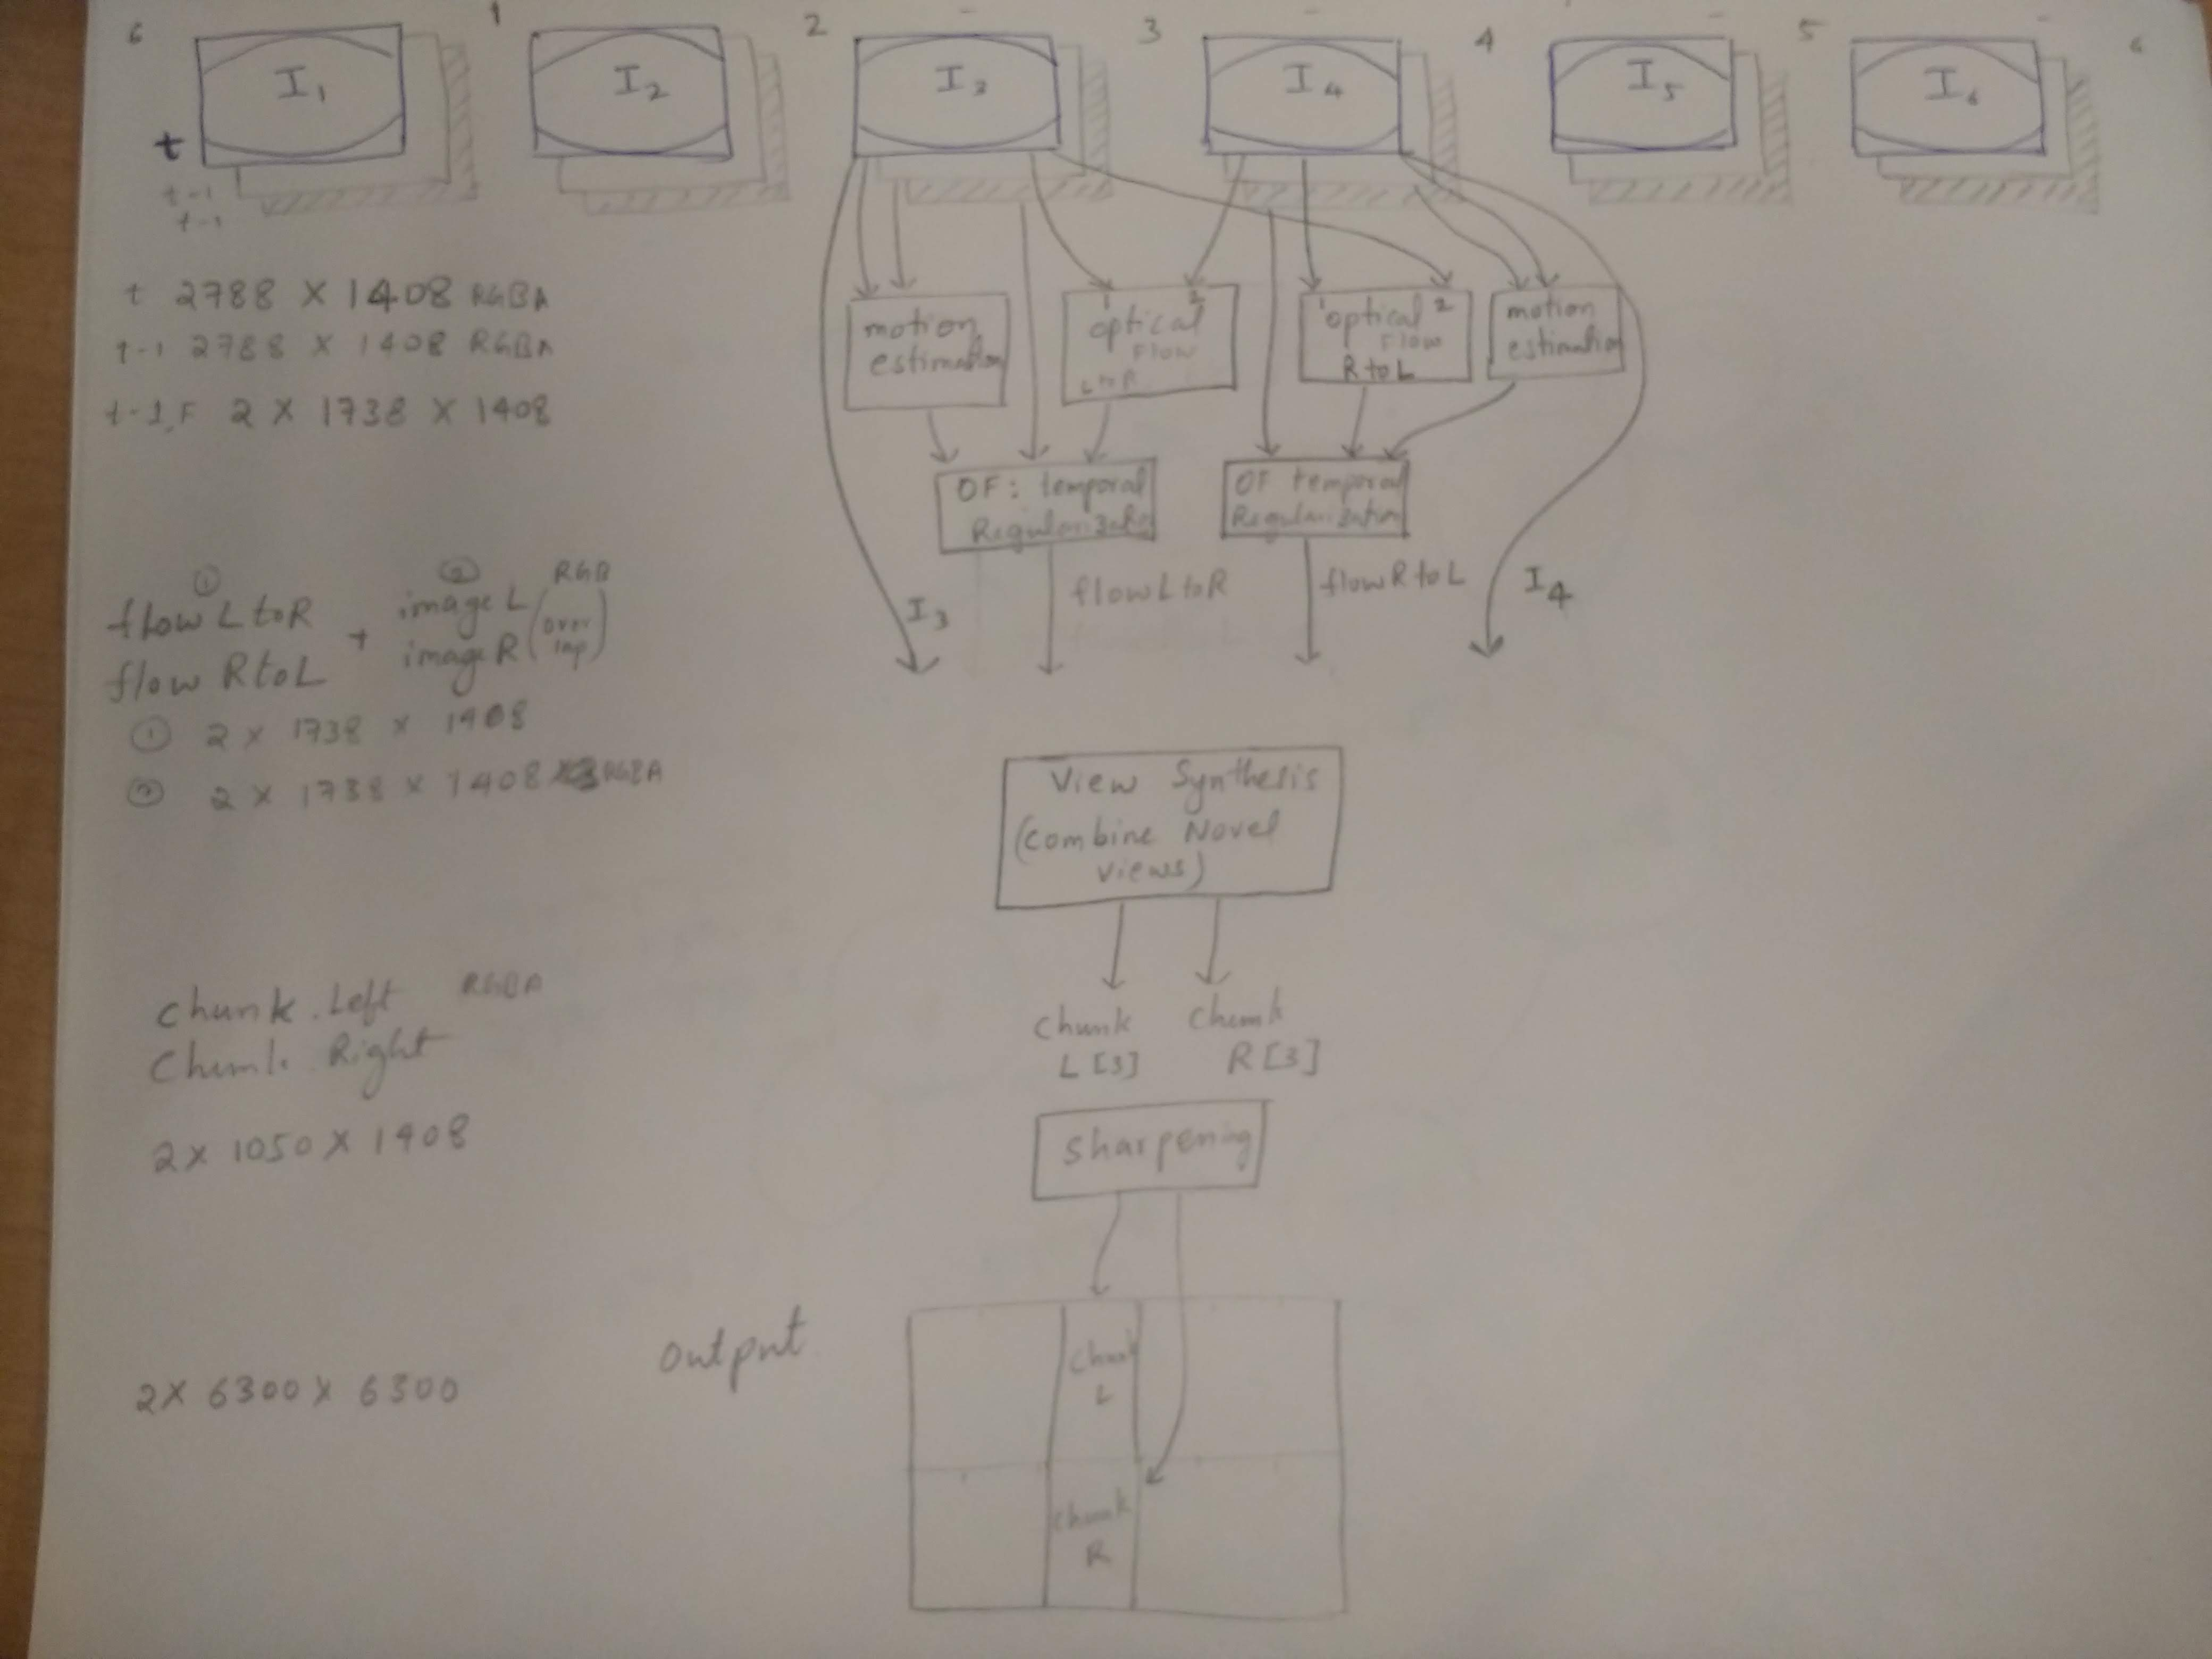
\includegraphics[width=1\textwidth]{/media/gunman/Data/thesis/ThesisLatex/data/images/ODS_Input_Output.jpg}
		\caption{X-axis shows the pyramid level and Y-axis the runtime tile search and propagate.}
		\label{ODS_Input_Output}
	\end{center}
	\vspace{-0.3in}
\end{figure*} 


\begin{figure*}
	\begin{center}
		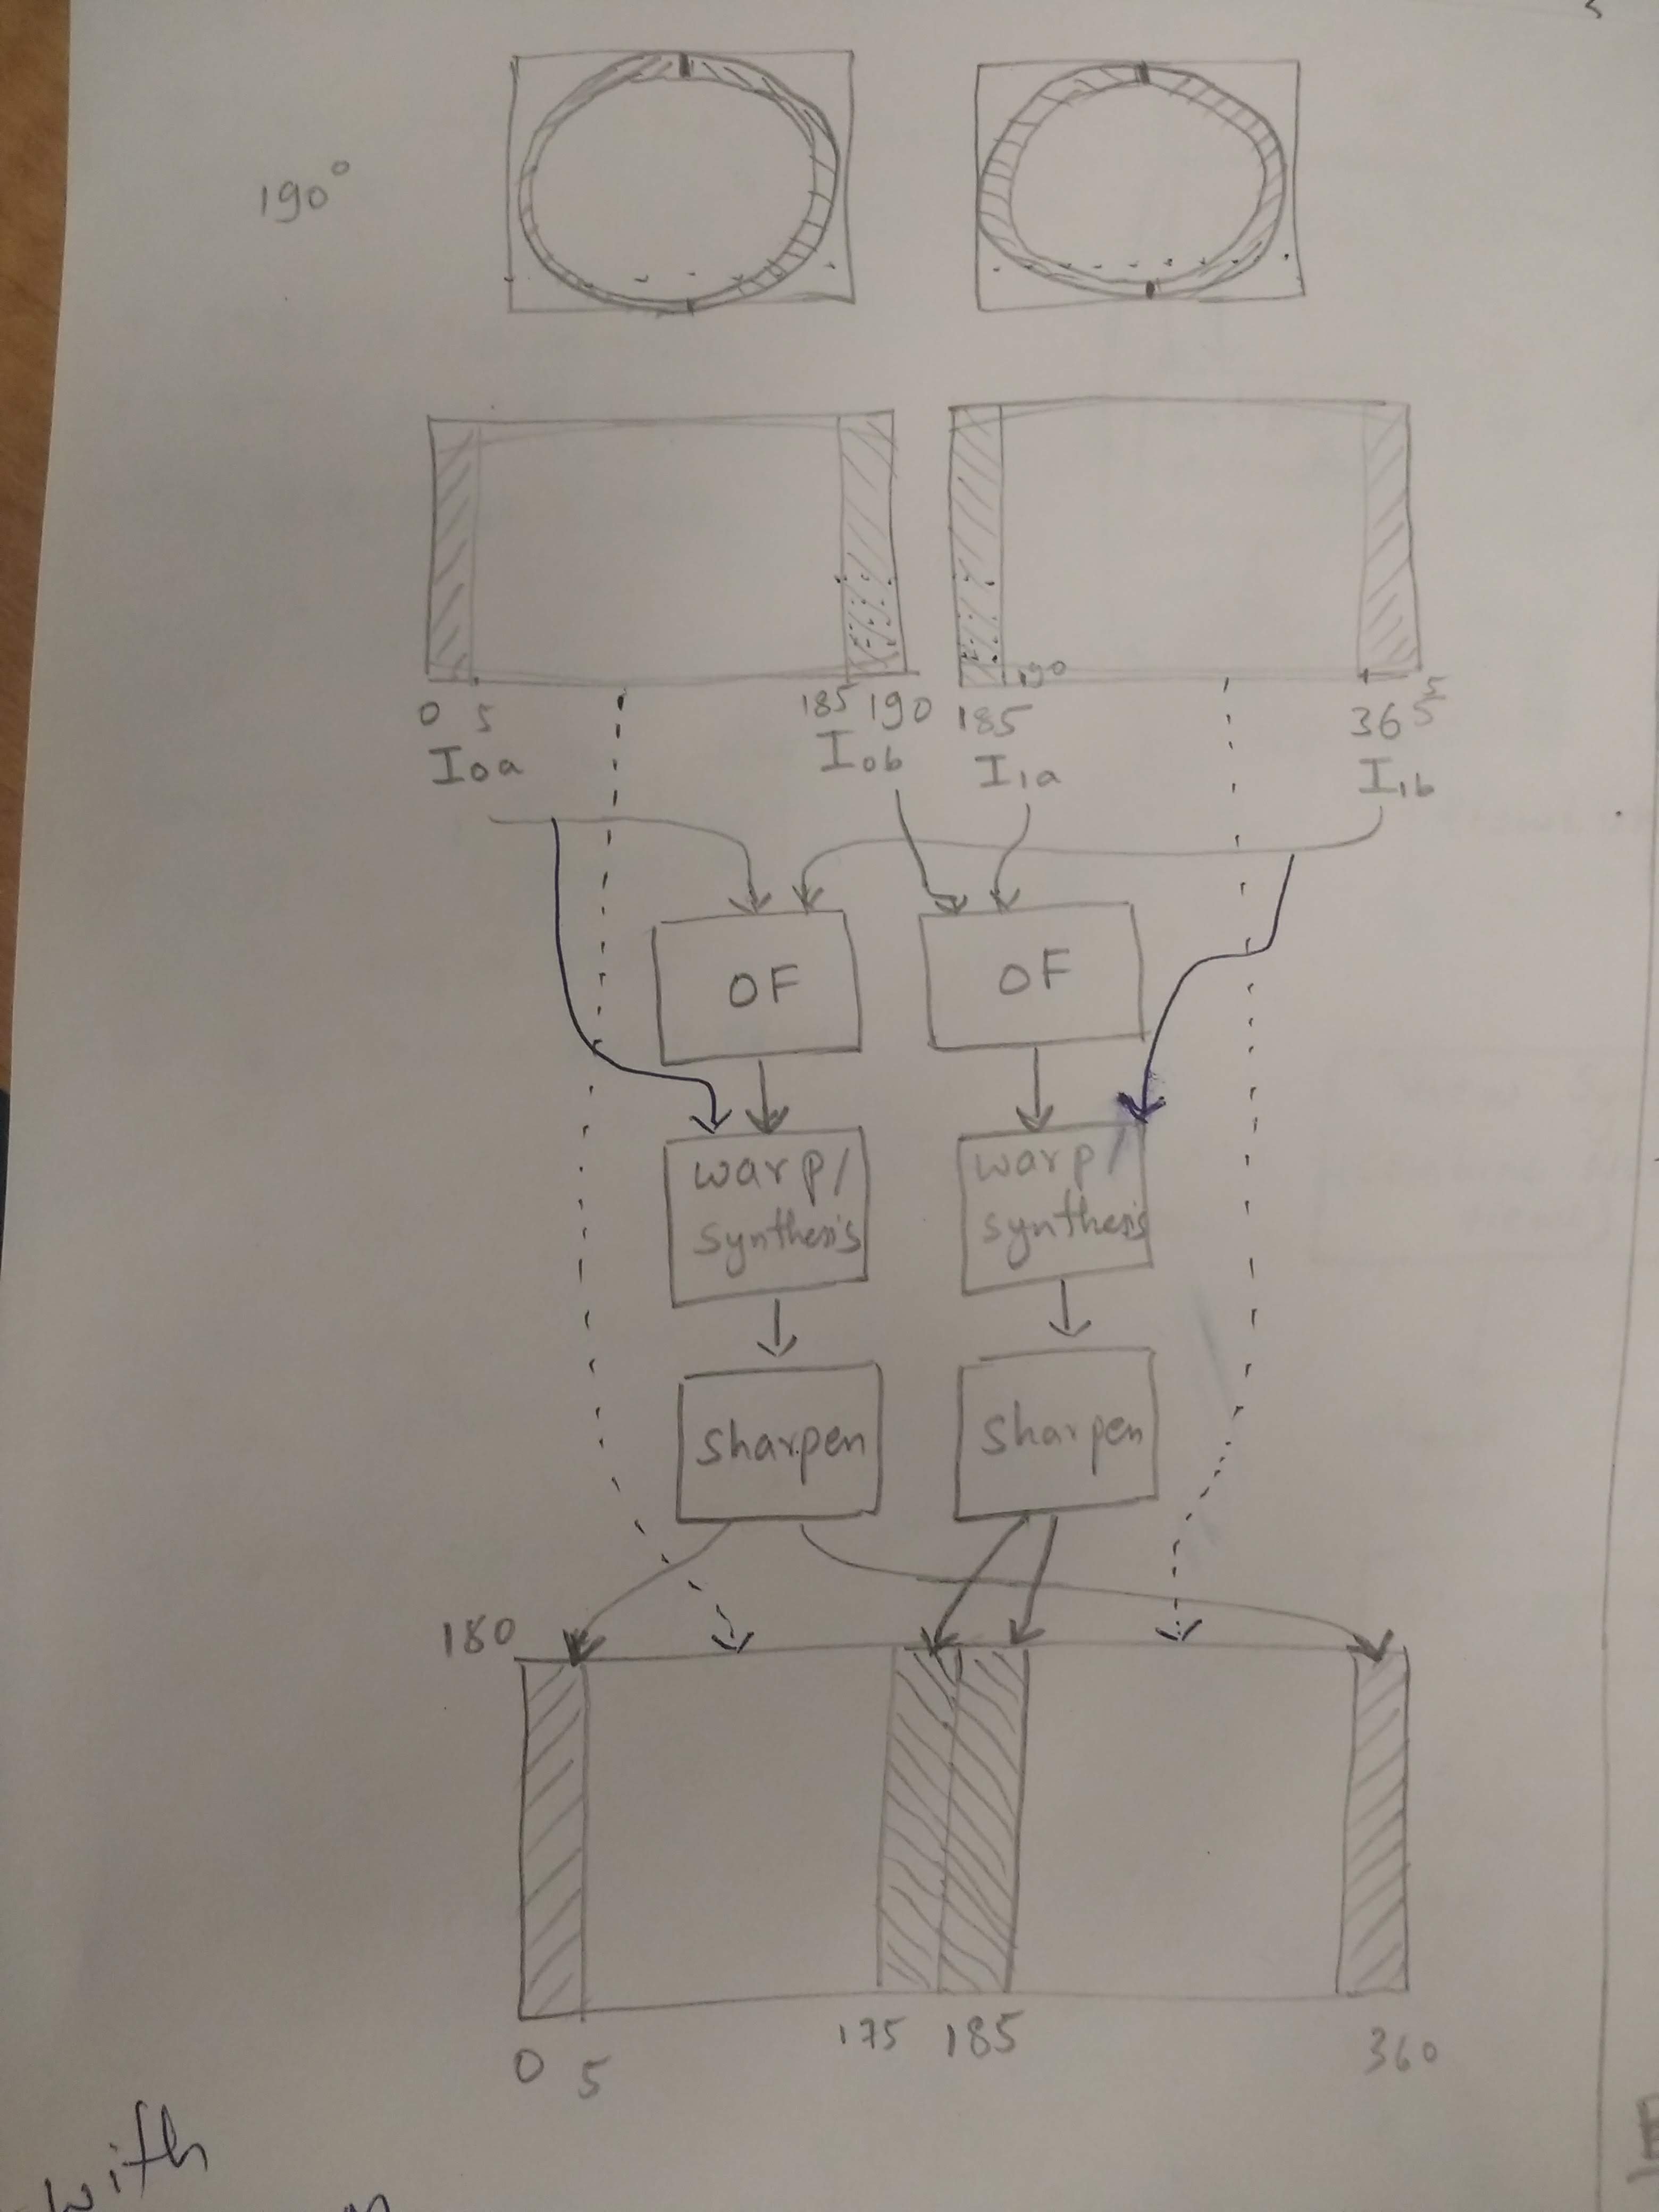
\includegraphics[width=1\textwidth]{/media/gunman/Data/thesis/ThesisLatex/data/images/Monoscopic_input_output.jpg}
		\caption{X-axis shows the pyramid level and Y-axis the runtime tile search and propagate.}
		\label{Monoscopic_Input_Output}
	\end{center}
	\vspace{-0.3in}
\end{figure*} 